\documentclass{article}
\usepackage[UTF8]{ctex} % Required for inserting images
\usepackage{graphicx}
\usepackage{amsmath}

\begin{document}

\section{作业二}

   \begin{figure}[!h]
       \centering
       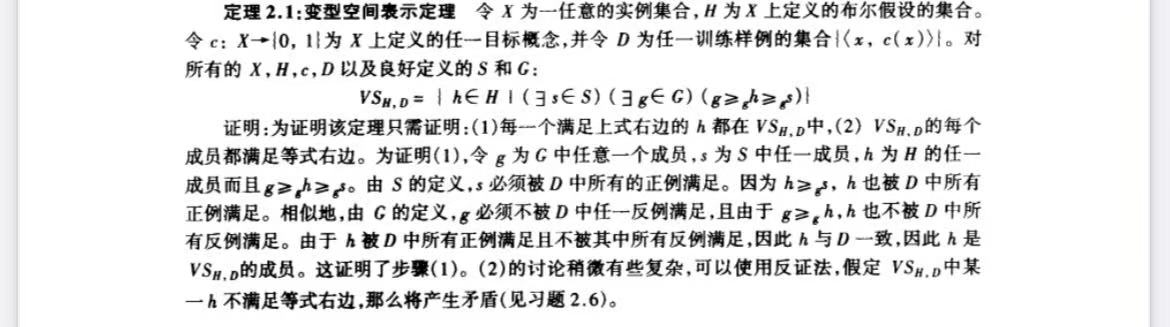
\includegraphics[width=1.2\linewidth]{image/2.6.jpg}
       \label{2.6}
   \end{figure}

    下面完成定理2.1第二部分的证明,即证明如果\(h\in V_{SH,D}\),则存在\(s\in S\)和\(g\in G\)使得\(g\geq h\geq s\)。
    
   \paragraph{基于反证法:}

    假设存在一个假设\(h\in V_{SH,D}\),\(h\)与训练数据\(D\)一致,但不存在\(s\in S\)和\(g\in G\)使得\(g\geq h\geq s\)。则可能有下面两种情况。

    \begin{enumerate}
       
        \item 对于所有\(s\in S\),都不满足\(h\geq s\),即\(h\)不比任何\(s\)一般或与之相等。
    
        \item 对于所有\(g\in G\),都不满足\(g\geq h\),即\(h\)不比任何\(g\)具体或与之相等。

    \end{enumerate}

    若假设成立上述状况至少其中一项成立。要证明假设不成立,则需要证明两种情况都不成立。

   \paragraph{情况1:}对于所有\(s\in S\),都不满足\(h\geq s\)
    
    由于\(h\)与\(D\)一致,它覆盖所有正例且不覆盖任何反例。
    
    \(S\)是变型空间中最具体的假设集合,即\(S\)中的每个假设都是与\(D\)一致的最具体的假设,不存在其他与\(D\)一致的假设比\(S\)中的假设更具体。

    若对于所有\(s\in S\),均不满足\(h\geq s\),那么\(h\)比每个\(s\in S\)更具体。因为\(h\)与\(D\)一致,且如果\(h\)更具体,则\(h\)可能仍然与\(D\)一致,与\(S\)的定义矛盾。
    
    若\(h\)比所有\(s\in S\)更具体且与\(D\)一致,那么\(h\)是最具体的假设之一,因此\(h\)应该属于\(S\),或至少存在某个\(s\in S\)使得\(s\leq h\)。与假设矛盾。
    
    情况1不成立。

    \paragraph{情况2:}对于所有\(g\in G\),都不满足\(g\geq h\)
    
    \(G\)是变型空间中最一般的假设集合,即\(G\)中的每个假设都是与\(D\)一致的最一般的假设,不能在其他与\(D\)一致的假设比\(G\)中的假设更一般。

    若对于所有\(g\in G\),均不满足\(g\geq h\),那么\(h\)比每个\(g\in G\)更一般。因为\(h\)与\(D\)一致,且如果\(h\)更一般,则\(h\)可能仍然与\(D\)一致,与\(G\)的定义矛盾。
    
    若\(h\)比所有\(g\in G\)更一般且与\(D\)一致,那么\(h\)是最一般的假设之一,因此\(h\)应该属于\(G\),或至少存在某个\(g\in G\)使得\(g\geq h\)。与假设矛盾。
    
    情况2不成立。

    由于两种情况都不成立,原假设不成立。则对于任何\(h\in V_{SH,D}\),必须存在\(s\in S\)和\(g\in G\)使得\(g\geq h\geq s\)。\\

    定理的第二部分证明完毕。

\end{document}